\documentclass[12pt]{article}
\usepackage{setspace, graphicx, fullpage, amssymb, amsmath, epsfig, natbib, array, multirow, hyperref}
\usepackage{amsfonts, bm} 
\usepackage{dcolumn}
\usepackage{subfigure, float} 
\usepackage[margin=1in]{geometry} 
\usepackage{verbatim}
\usepackage{url}
\usepackage{enumerate}
\newcolumntype{d}[1]{D{.}{.}{#1}} 

\begin{document}
	
	\begin{center}
		Update: 11 January 2017
	\end{center}

In the last week I have focused on the Senate data since I recognized too late that we did not have data on retirement or committee assignments readily available for House 110 - 112. I found what I believe to have been the causes of cases dropping from the previous method for building Senator year data which William and I were building this previously. It appears that the way the current package handled Senators who had served discontinuous terms had caused them to be removed by other parts of the script. When these parts of the script were adjusted, these individuals remained in the data. These updated scripts were partly relied upon in the process of getting the data built with the LES data we got from Alan. 

The first set of tables included are summary stats for the variables used in our Senate models (along with a few extras) from this data, separated by party. Additionally, I have used this data to rerun the Senate tables for the \verb|emIRT| only sorting algorithm. I find that initially, high collinearity between presidential vote share seems to hide the relationship between ideological extremism and responsiveness to party calls for Democrats. This carries over into the majority model (though not the minority model). However, removing this variable from the model does not change  Unfortunately, looking at the figure this produces shows that this problem holds across our data as it is now.

As it stands, my plan for the coming week is to get the House data we need to finish the package and to try to determine if there is something throwing off our Senate figures. The former I am confident in my ability to do (given enough time) and guidance would be appreciated on the latter. Please let me know if any of the summary statistic values look particularly odd to you (for instance, 70\% of members serving on a Senate power committee seems fairly high to me). Alternatively, if you have other variables you think I would be wise to investigate for other reasons I would appreciate guidance on that as well.

% Table created by stargazer v.5.2 by Marek Hlavac, Harvard University. E-mail: hlavac at fas.harvard.edu
% Date and time: Tue, Jan 10, 2017 - 18:08:47
\begin{table}[!htbp] \centering 
	\label{} 
	\begin{tabular}{@{\extracolsep{5pt}}lcc} 
		\\[-1.8ex]\hline 
		\hline \\[-1.8ex] 
		Statistic & \multicolumn{1}{c}{Mean} & \multicolumn{1}{c}{St. Dev.} \\ 
		\hline \\[-1.8ex] 
		class & 1.954 & 0.846 \\ 
		pres\_vote\_share & 0.485 & 0.093 \\ 
		votepct & 60.596 & 9.735 \\ 
		south & 0.233 & 0.423 \\ 
		south11 & 0.212 & 0.409 \\ 
		south13 & 0.236 & 0.425 \\ 
		south17 & 0.342 & 0.475 \\ 
		leader & 0.082 & 0.274 \\ 
		chair & 0.180 & 0.385 \\ 
		best\_committee & 3.767 & 2.738 \\ 
		power\_committee & 0.722 & 0.448 \\ 
		up\_for\_reelection & 0.334 & 0.472 \\ 
		freshman & 0.333 & 0.471 \\ 
		superfreshman & 0.023 & 0.152 \\ 
		seniority & 5.704 & 4.963 \\ 
		retiree & 0.061 & 0.240 \\ 
		afam & 0.006 & 0.075 \\ 
		female & 0.086 & 0.281 \\ 
		latino & 0.007 & 0.081 \\ 
		gingrich\_senator & 0.000 & 0.000 \\ 
		maj & 0.631 & 0.483 \\ 
		party\_free\_ideal\_point & $-$0.791 & 0.520 \\ 
		pirate100 & 82.572 & 12.211 \\ 
		pfrate100 & 84.130 & 10.074 \\ 
		ideological\_extremism & 0.791 & 0.520 \\ 
		\hline \\[-1.8ex] 
	\end{tabular} 
	\caption{Senate Data emIRT Only, Democrat Summary Stats} 
\end{table} 

% Table created by stargazer v.5.2 by Marek Hlavac, Harvard University. E-mail: hlavac at fas.harvard.edu
% Date and time: Tue, Jan 10, 2017 - 18:10:48
\begin{table}[!htbp] \centering 
	\label{} 
	\begin{tabular}{@{\extracolsep{5pt}}lcc} 
		\\[-1.8ex]\hline 
		\hline \\[-1.8ex] 
		Statistic & \multicolumn{1}{c}{Mean} & \multicolumn{1}{c}{St. Dev.} \\ 
		\hline \\[-1.8ex] 
		class & 2.051 & 0.787 \\ 
		pres\_vote\_share & 0.562 & 0.085 \\ 
		votepct & 59.002 & 9.121 \\ 
		south & 0.275 & 0.447 \\ 
		south11 & 0.225 & 0.418 \\ 
		south13 & 0.282 & 0.450 \\ 
		south17 & 0.335 & 0.472 \\ 
		leader & 0.115 & 0.319 \\ 
		chair & 0.139 & 0.346 \\ 
		best\_committee & 3.710 & 2.620 \\ 
		power\_committee & 0.717 & 0.451 \\ 
		up\_for\_reelection & 0.328 & 0.470 \\ 
		freshman & 0.389 & 0.488 \\ 
		superfreshman & 0.014 & 0.120 \\ 
		seniority & 4.605 & 4.172 \\ 
		retiree & 0.058 & 0.234 \\ 
		afam & 0.003 & 0.056 \\ 
		female & 0.051 & 0.220 \\ 
		latino & 0.007 & 0.085 \\ 
		gingrich\_senator & 0.198 & 0.398 \\ 
		maj & 0.474 & 0.500 \\ 
		party\_free\_ideal\_point & 0.870 & 0.588 \\ 
		pirate100 & 83.302 & 12.551 \\ 
		pfrate100 & 81.904 & 10.166 \\ 
		ideological\_extremism & 0.865 & 0.595 \\ 
		\hline \\[-1.8ex] 
	\end{tabular} 
	\caption{Senate Data emIRT Only, Republican Summary Stats}
\end{table} 

\begin{table}
	\begin{center}
		\begin{tabular}{l c c c c }
			\hline
			& Democrats & Republicans & Majority & Minority \\
			\hline
			(Intercept)            & $6.886^{*}$    & $4.288$       & $0.295$        & $1.220$        \\
			& $(3.311)$      & $(3.128)$     & $(3.336)$      & $(3.399)$      \\
			ideological\_extremism & $-4.014^{***}$ & $2.569^{***}$ & $-1.481^{*}$   & $1.368^{*}$    \\
			& $(0.688)$      & $(0.534)$     & $(0.657)$      & $(0.579)$      \\
			pfrate100              & $0.836^{***}$  & $0.905^{***}$ & $0.887^{***}$  & $0.889^{***}$  \\
			& $(0.034)$      & $(0.030)$     & $(0.034)$      & $(0.033)$      \\
			pres\_vote\_share      & $29.705^{***}$ & $-4.299$      & $15.311^{***}$ & $17.827^{***}$ \\
			& $(2.850)$      & $(3.122)$     & $(2.549)$      & $(2.998)$      \\
			south                  & $-3.471^{***}$ & $0.227$       & $0.516$        & $-1.484^{*}$   \\
			& $(0.633)$      & $(0.584)$     & $(0.549)$      & $(0.606)$      \\
			votepct                & $-0.055^{*}$   & $0.046$       & $0.015$        & $-0.032$       \\
			& $(0.027)$      & $(0.030)$     & $(0.028)$      & $(0.029)$      \\
			female                 & $-0.470$       & $1.381$       & $-0.301$       & $2.374^{*}$    \\
			& $(0.853)$      & $(1.117)$     & $(0.952)$      & $(1.057)$      \\
			afam                   & $4.041$        & $-7.168$      & $1.147$        & $-1.698$       \\
			& $(2.982)$      & $(4.328)$     & $(4.339)$      & $(3.095)$      \\
			latino                 & $-1.028$       & $-5.643^{*}$  & $-1.741$       & $-2.381$       \\
			& $(2.738)$      & $(2.807)$     & $(2.502)$      & $(3.383)$      \\
			up\_for\_reelection    & $-0.762$       & $-0.028$      & $0.054$        & $-1.335^{*}$   \\
			& $(0.499)$      & $(0.555)$     & $(0.521)$      & $(0.594)$      \\
			seniority              & $0.018$        & $0.139$       & $0.118$        & $0.093$        \\
			& $(0.071)$      & $(0.085)$     & $(0.087)$      & $(0.077)$      \\
			freshman               & $-0.505$       & $0.539$       & $0.899$        & $0.504$        \\
			& $(0.676)$      & $(0.785)$     & $(0.722)$      & $(0.787)$      \\
			retiree                & $1.857$        & $-0.552$      & $1.405$        & $0.947$        \\
			& $(1.023)$      & $(1.087)$     & $(1.148)$      & $(1.070)$      \\
			best\_committee        & $-0.181$       & $0.182$       & $-0.049$       & $-0.046$       \\
			& $(0.150)$      & $(0.166)$     & $(0.156)$      & $(0.177)$      \\
			leader                 & $-0.911$       & $0.149$       & $0.231$        & $-0.466$       \\
			& $(0.843)$      & $(0.789)$     & $(0.843)$      & $(0.871)$      \\
			power\_committee       & $-0.331$       & $1.399$       & $0.466$        & $0.223$        \\
			& $(0.905)$      & $(0.937)$     & $(0.915)$      & $(1.031)$      \\
			chair                  & $-1.889^{**}$  & $-1.953^{**}$ & $-1.894^{**}$  & $-8.374$       \\
			& $(0.678)$      & $(0.741)$     & $(0.674)$      & $(7.548)$      \\
			\hline
			R$^2$                  & 0.630          & 0.666         & 0.587          & 0.662          \\
			Adj. R$^2$             & 0.624          & 0.660         & 0.581          & 0.656          \\
			Num. obs.              & 1037           & 948           & 1047           & 839            \\
			RMSE                   & 7.151          & 7.321         & 7.413          & 7.451          \\
			\hline
			\multicolumn{5}{l}{\scriptsize{$^{***}p<0.001$, $^{**}p<0.01$, $^*p<0.05$}}
		\end{tabular}
	\caption{Senate Models, emIRT Only}
\end{center}
\end{table}

\begin{table}
	\begin{center}
		\begin{tabular}{l c c c c }
			\hline
			& Democrats & Republicans & Majority & Minority \\
			\hline
			(Intercept)            & $8.767^{*}$    & $2.422$       & $3.813$       & $9.210^{**}$  \\
			& $(3.476)$      & $(2.820)$     & $(3.340)$     & $(3.187)$     \\
			ideological\_extremism & $-2.949^{***}$ & $2.337^{***}$ & $-0.538$      & $2.181^{***}$ \\
			& $(0.715)$      & $(0.507)$     & $(0.649)$     & $(0.574)$     \\
			pfrate100              & $0.919^{***}$  & $0.908^{***}$ & $0.903^{***}$ & $0.885^{***}$ \\
			& $(0.035)$      & $(0.030)$     & $(0.034)$     & $(0.033)$     \\
			south                  & $-3.498^{***}$ & $0.283$       & $0.242$       & $-1.470^{*}$  \\
			& $(0.665)$      & $(0.583)$     & $(0.556)$     & $(0.619)$     \\
			votepct                & $-0.000$       & $0.037$       & $0.047$       & $-0.016$      \\
			& $(0.027)$      & $(0.029)$     & $(0.028)$     & $(0.030)$     \\
			female                 & $1.317$        & $1.482$       & $0.201$       & $2.646^{*}$   \\
			& $(0.879)$      & $(1.115)$     & $(0.964)$     & $(1.077)$     \\
			afam                   & $5.055$        & $-6.972$      & $1.308$       & $-1.544$      \\
			& $(3.133)$      & $(4.328)$     & $(4.412)$     & $(3.159)$     \\
			latino                 & $-0.752$       & $-5.460$      & $-1.880$      & $-2.953$      \\
			& $(2.879)$      & $(2.805)$     & $(2.544)$     & $(3.452)$     \\
			up\_for\_reelection    & $-0.758$       & $-0.062$      & $0.142$       & $-1.373^{*}$  \\
			& $(0.524)$      & $(0.555)$     & $(0.529)$     & $(0.606)$     \\
			seniority              & $0.159^{*}$    & $0.145$       & $0.097$       & $0.112$       \\
			& $(0.073)$      & $(0.085)$     & $(0.088)$     & $(0.079)$     \\
			freshman               & $0.414$        & $0.566$       & $1.257$       & $0.584$       \\
			& $(0.705)$      & $(0.785)$     & $(0.732)$     & $(0.803)$     \\
			retiree                & $2.549^{*}$    & $-0.491$      & $1.476$       & $1.008$       \\
			& $(1.073)$      & $(1.086)$     & $(1.168)$     & $(1.092)$     \\
			best\_committee        & $-0.132$       & $0.162$       & $-0.042$      & $-0.017$      \\
			& $(0.158)$      & $(0.165)$     & $(0.158)$     & $(0.181)$     \\
			leader                 & $-1.604$       & $0.111$       & $0.453$       & $-0.358$      \\
			& $(0.883)$      & $(0.789)$     & $(0.857)$     & $(0.889)$     \\
			power\_committee       & $-0.299$       & $1.355$       & $0.547$       & $0.129$       \\
			& $(0.951)$      & $(0.936)$     & $(0.930)$     & $(1.052)$     \\
			chair                  & $-2.515^{***}$ & $-1.958^{**}$ & $-1.528^{*}$  & $-6.120$      \\
			& $(0.710)$      & $(0.741)$     & $(0.682)$     & $(7.695)$     \\
			\hline
			R$^2$                  & 0.591          & 0.665         & 0.573         & 0.648         \\
			Adj. R$^2$             & 0.585          & 0.660         & 0.567         & 0.641         \\
			Num. obs.              & 1037           & 948           & 1047          & 839           \\
			RMSE                   & 7.519          & 7.324         & 7.538         & 7.605         \\
			\hline
			\multicolumn{5}{l}{\scriptsize{$^{***}p<0.001$, $^{**}p<0.01$, $^*p<0.05$}}
		\end{tabular}
		\caption{Statistical models}
		\label{table:coefficients}
	\end{center}
\end{table}
			
			

\begin{figure}[h]
	\caption{Figure 2, Ideological Extremism, Senate emIRT Only}
	\centering
	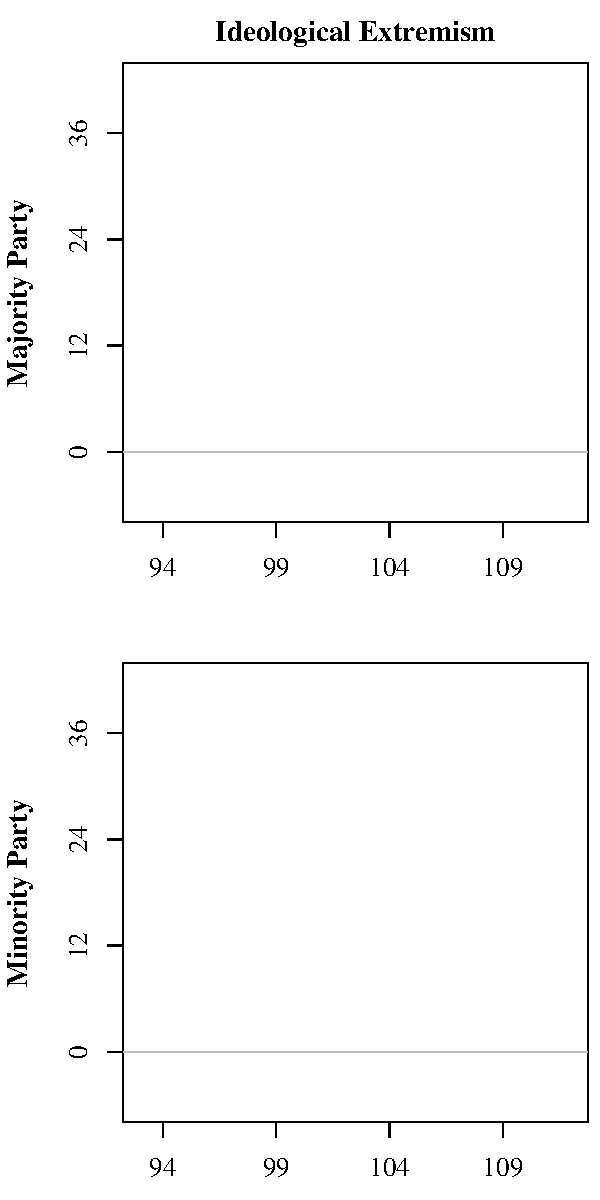
\includegraphics[]{C:/Users/Ethan/Documents/GitHub/partycalls/plots/senate-figure2-emIRT_only.pdf}
	
\end{figure}	
			

















\end{document}